\section{Ambiente virtual}

O Unity 3D é uma das ferramentas mais usadas para criar jogos para as mais diversas 
plataformas, e diferente do que muitos acreditam o software pode ser muito simples 
de usar quando se conhece o seu funcionamento básico. É possível criar jogos e 
aplicações interativas no Unity para Web, Desktop, iOS, Android e até mesmo 
consoles como PS3, XBOX 360 e Wii.

Para iniciar a modelagem do Parque Virtual foi escolhido um mapa em escala de 
cinza para que sirva de base para o ambiente virtual. O mapa foi adaptado para 
que fosse reconhecido pelo Unity.

\begin{figure}[htpb]
 \begin{center}
    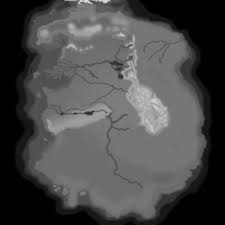
\includegraphics[width=.40\textwidth]{figuras/mapa.jpeg}
 \end{center}
  \caption{Mapa do ambiente virtual em escala de cinza}
  \label{fig:core_concurrent}
\end{figure}

O mapa foi importado para o Unity e foi colocada nele uma base de grama para que
os outros componentes sejam colocadas por cima desta base.

Foi feita uma adequação do terreno formado pelo mapa de cores para que fosse criada
a ciclovia.
 

Falar um pouco de como esta sendo modelado o ambiente virtual: mostrar o mapa de altura (imagem), quais recursos a serem adicionados no ambiente (tunel, ponte, caichoeira, etc)
